\parindent=0em
\section{Dispositivos}
\noindent

%https://editeca.com/realidad-mixta/
Dado que la realidad aumentada y la realidad virtual tienen distintas necesidades tecnológicas como se ha tratado en la sección~\ref{sec:necesidadesTecnologicas}, sus dispositivos correspondientes también tienen componentes hardware distintos para satisfacer estas necesidades tecnológicas.\\

En el sector de la realidad aumentada destaca principalmente el uso de teléfonos móviles gracias a su fácil disponibilidad y a la facilidad añadida de crear aplicaciones para estos gracias a la aparición de las tecnologías ARCore y ARKit. Se puede disfrutar de esta experiencia usando gafas de realidad aumentada y HMDs.\\

Por otra parte, en el campo de la realidad virtual destacan los HMD. Estos dispositivos son variados entre ellos en cuanto a los sensores, cámaras o conectividad entre otras características.\\

Al ser la realidad mixta una combinación entre las dos realidades mencionadas anteriormente, la MR puede ser utilizada a través de cascos enfocados a experiencias de realidad virtual (aunque estos cascos no se van a tratar en esta sección), dispositivos enfocados para su uso en realidad aumentada o incluso desde teléfonos móviles.\\

Del mismo modo, se pueden distinguir dos tipos de dispositivos específicos de realidad mixta en el campo de los HMD. Por un lado los cascos en los que se ve directamente el mundo físico y por otro aquellos HMD en los que la visión del usuario está completamente tapada por el casco y el mundo real se ve a través de las cámaras del dispositivo.\\

%https://www.microsoft.com/en-us/mixed-reality/windows-mixed-reality?rtc=1


También, cabe destacar que un gran número de dispositivos de realidad mixta se utilizan a través de la plataforma WMR\footnotemark~  (\textit{Windows Mixed Reality}). Esta plataforma ofrece acceso a numerosas aplicaciones de realidad mixta y realidad virtual. Para poder hacer uso de WMR es necesario un ordenador con Windows~10 y una tarjeta gráfica y procesador potentes ya que los HMD utilizan dichos componentes para funcionar.\\

\footnotetext{\url{https://www.microsoft.com/en-us/mixed-reality/windows-mixed-reality}}


Por último, los teléfonos móviles están empezando a ganar importancia en el sector de la realidad mixta. Según un estudio realizado por Sam Barker \cite{juniperArMrmoney}, los avances en el \textit{Edge Computing}~\cite{edgeComputing}, un paradigma que permite que los servicios de computación en la nube~\cite{cloudComputing} (tecnología de computación que provee unidades computacionales de bajo coste) sean más cercanos al usuario final, y la aparición de las redes de 5G (la quinta generación de tecnología inalámbrica la cual se caracteriza por un aumento de la velocidad y menor latencia frente al 4G), acelerarán el desarrollo de la tecnología de realidad mixta en móviles.\\

Dicho autor afirma que las conexiones inalámbricas que se utilizan hoy día para procesar la información de los dispositivos, deberán alcanzar velocidades mayores (usando el 5G) para una experiencia inmersiva total. En este estudio se calcula que gracias a estos avances se alcanzará un mercado de~43 billones de dólares en el año~2024, a diferencia de los 8 billones alcanzados en~2019.

\parindent=0em
\subsection{Teléfonos móviles}
\label{sec:telefonosMoviles}
\noindent

%https://www.aniwaa.com/product/vr-ar/tesseract-holoboard-enterprise-edition/

Los teléfonos móviles son un gran dispositivo ya que combinan GPS, cámara, brújula y un acelerómetro, cubriendo así las necesidades de una aplicación de realidad aumentada~\cite{arsmartphones}. El teléfono móvil es un dispositivo muy común entre la población lo cual facilita el desarrollo y expansión de esta realidad. Por otro lado, dichos dispositivos se pueden utilizar también para realidad mixta utilizando unos cascos en los que se introduce el móvil para generar una experiencia de MR.\\

Existen distintos HMD que se utilizan para estas experiencias de realidad mixta acoplando los móviles a alguna parte de las gafas, como por ejemplo, las \textit{Holoboard Enterprise Edition} de la mano de la empresa \textit{TESSERACT} (figura~\ref{fig:mrandroidTESSERACT}). Este dispositivo es compatible a partir de Android 6.0  y como especificaciones técnicas se pueden destacar sus 82\degree~ de FOV, utiliza la tecnología SLAM para el \textit{tracking}, posee un controlador 6DoF y utiliza el \textit{tracking} por sensores IMU, además, permite experiencias colaborativas en la nube.

\begin{figure}[H]
    \centering
    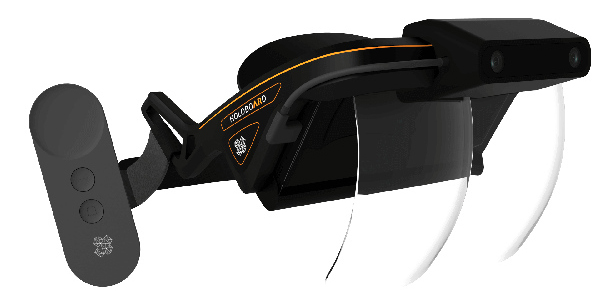
\includegraphics[scale=0.3]{Images/Estado del arte/mrandroid.jpg}
    \caption[\textit{Holoboard Enterprise Edition}]{
    \textit{Holoboard Enterprise Edition\footnotemark.}
    }
    \label{fig:mrandroidTESSERACT}
\end{figure}
\footnotetext{Fuente: \url{https://www.aniwaa.com/product/vr-ar/tesseract-holoboard-enterprise-edition}}
En cambio, si estamos hablando de un dispositivo para utilizar en móviles con iOS podemos hablar del casco \textit{Bridge} (figura~\ref{fig:mriosBRIDGE}) de la empresa \textit{Occipital}. Este HMD requiere de un componente extra llamado \textit{Occipital Structure Sensor}, el cual, se utiliza para el escaneo 3D del entorno.

\begin{figure}[H]
    \centering
    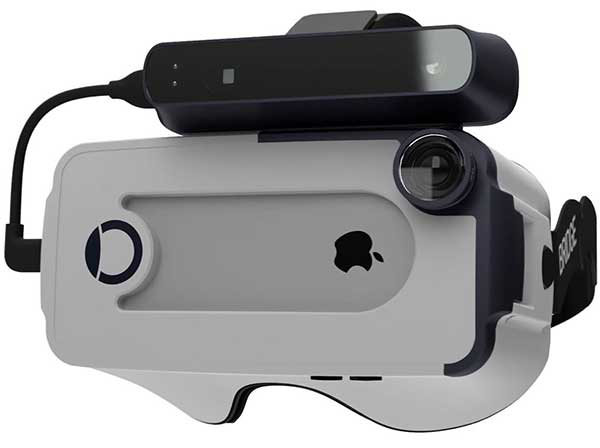
\includegraphics[scale=0.3]{Images/Estado del arte/mrios.jpg}
    \caption[\textit{Occipital Bridge}]{\textit{Occipital Bridge\footnotemark.}}
    \label{fig:mriosBRIDGE}
\end{figure}

\footnotetext{Fuente: \url{https://www.aniwaa.com/product/vr-headsets/occipital-bridge/}}

Las gafas \textit{Bridge} tienen un FOV de 120º, un controlador de 6DoF y destacan por que gracias a estas se puede utilizar aplicaciones de realidad aumentada, realidad mixta y realidad virtual, también, utiliza la técnica de \textit{tracking} conocida como \textit{inside-out}.\\

Pese a que la principal diferencia entre las dos gafas es el sistema operativo para el que están destinadas, se puede observar que los precios son similares y que las gafas destinadas para iOS poseen un FOV notablemente superior.


\begin{table}[H]
\centering
\renewcommand{\arraystretch}{1.5}
\begin{tabular}{llllll}
\toprule
Dispositivo                  & Precio & DoF & FOV & \textit{SO} & \textit{Tracking} \\
\midrule
\textit{Holoboard Enterprise Edition} & \$399  & 6DoF         & 82\degree           & Android     & SLAM              \\
\textit{Occipital Bridge }            & \$349  & 6DoF         & 120\degree          & iOS         & \textit{Inside-out}\\\bottomrule       
\end{tabular}
\caption{Comparación entre ambas gafas de \textit{MR} para móviles.}
\label{cuadro:comparacionphonesMR}
\end{table}


\parindent=0em
\subsection{Hololens 2}
\label{HoloLens2Dispositivo}
\noindent

Las \textit{HoloLens 2} (figura~\ref{fig:vistasHoloLens2}) son un casco desarrollado por \textit{Microsoft} que salió al mercado en 2019. Es un dispositivo dotado de tecnología de \textit{eye tracking} y \textit{hand tracking} capaz de detectar las dos manos, esto añade un extra de inmersión a la experiencia y de comodidad ya que no se necesitan mandos para manejarlo y se pueden tener las manos libres. Respecto a los sensores, goza de acelerómetro, giroscopio y magnetómetro para medir la velocidad, orientación y fuerzas gravitacionales del dispositivo.\\


\begin{figure}[htbp]
\centering
    \hspace{-4mm}
    \begin{minipage}{0.5\textwidth}
        \centering
        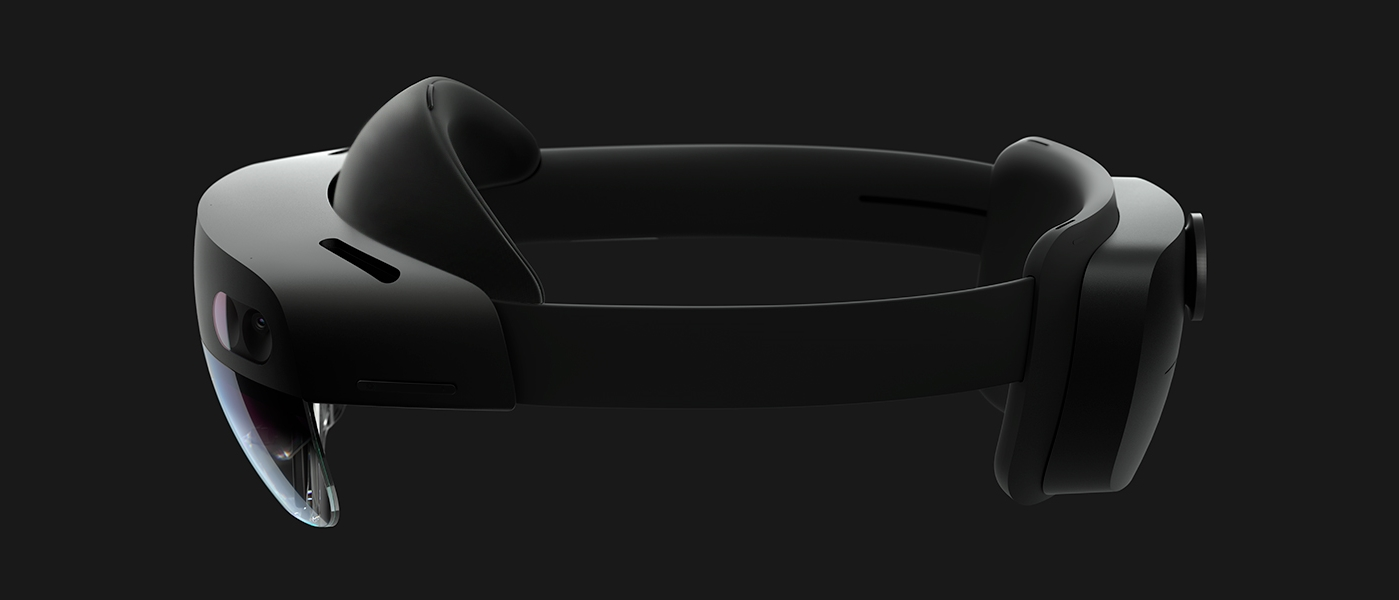
\includegraphics[scale=0.2]{Images/Estado del arte/hololens2_2.jpeg}\\
        (a) Vista lateral.
    \end{minipage}
    \begin{minipage}{0.5\textwidth}
        \centering
        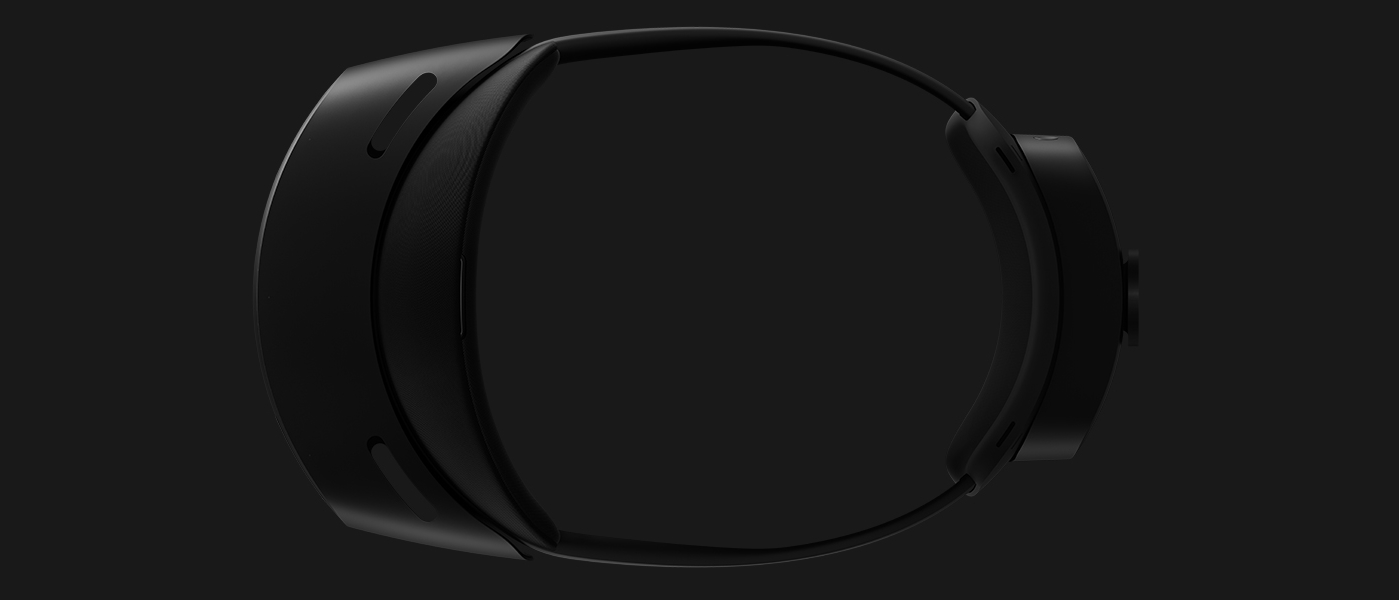
\includegraphics[scale=0.2]{Images/Estado del arte/hololens2_3.jpeg}\\
       (b) Vista superior.
    \end{minipage}\\
    \caption{Vistas de las Microsoft HoloLens 2\textsuperscript{\ref{hololens2footer}}.}
    \label{fig:vistasHoloLens2}
\end{figure}


Las \textit{Hololens 2} funcionan de forma independiente ya que tienen integrado su propio procesador y utilizan una batería recargable con una autonomía de entre 2 y 3 horas, además, permiten capturar el movimiento y los giros del usuario gracias a su control de \textit{6DoF}. Por otra parte, respecto a la conectividad, este \textit{HMD} tiene \textit{WiFi}, \textit{bluetooth} y permite conexiones mediante un \textit{USB} tipo C. Por ejemplo, se puede utilizar la conexión \textit{WiFi} para navegar por internet (a través del navegador \textit{Microsoft Edge} incorporado en las gafas) o para conectarse a reuniones en línea con otros usuarios de las mismas gafas.\\

Del mismo modo, este casco  está diseñado con un sistema ergonómico de tal forma que no hay necesidad de quitarse las gafas, ya que se puede colocar directamente sobre ellas (figura~\ref{fig:hololensErgonomicas}).\\


\begin{figure}[H]
    \centering
    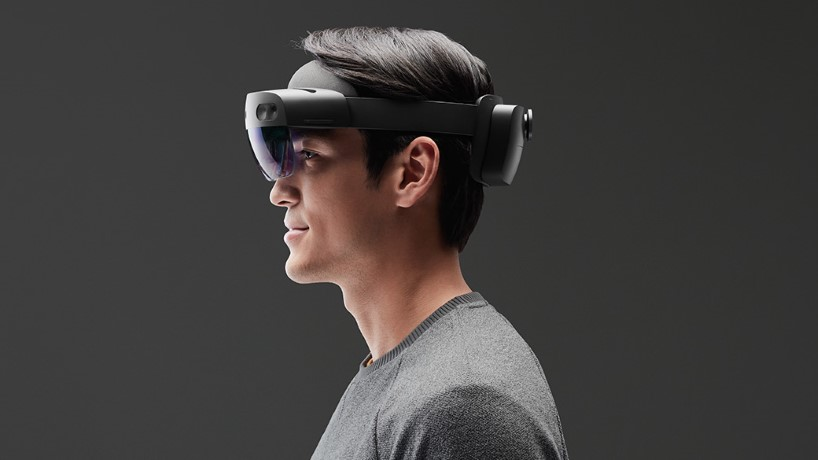
\includegraphics[scale=0.35]{Images/Estado del arte/hololens2_1.jpeg}
     \caption{Diseño ergonómico del dispositivo\textsuperscript{\ref{hololens2footer}}.
  }
  \label{fig:hololensErgonomicas}
\end{figure}


Para finalizar, este \textit{HMD} tiene un \textit{FOV} de 43º, una resolución de 2.048×1.080 píxeles por ojo (4.096x1.080 en combinación) y una \textit{IPD} que se ajusta automáticamente según la posición de los ojos que es detectada por un sensor \textit{IPD}, asimismo, tiene un sensor de~1~Megapíxel de profundidad \textit{ToF} (del inglés Time of Flight, calcula distancias entre objetos en función a la distancia que tarda la emisión y recepción de un haz de luz infrarrojo) y un peso de 566 gramos.  


%https://www.microsoft.com/es-es/hololens/hardware



\parindent=0em
\subsection{HMD Odyssey+}
\label{sec:odyssey}
\noindent

%https://www.samsung.com/hk_en/news/product/reality-headset-hmd-odyssey-plus/

El casco \textit{HDM Odyssey+} (figura~\ref{fig:hdmOdysseyVista}) es un dispositivo desarrollado por la empresa \textit{Samsung} que salió al mercado en 2018, no es un casco independiente ya que requiere estar conectado a un ordenador compatible con la plataforma \textit{Windows Mixed Reality} para funcionar, se conecta al ordenador mediante un cable \textit{HDMI}~2.0 y un \textit{USB}~3.0.

\begin{figure}[h]
    \centering
    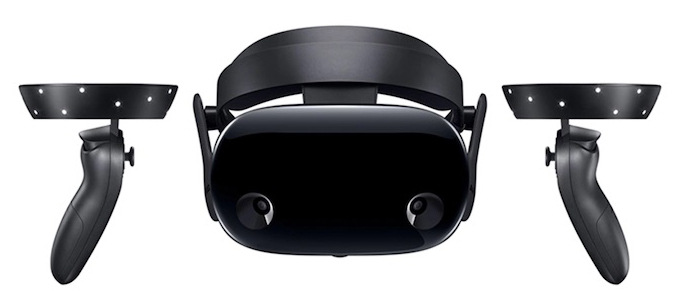
\includegraphics[scale=0.6]{Images/Estado del arte/samsungOdysseyplus.jpg}
    \caption{HDM Odyssey+ dispositivo al completo.}
    \label{fig:hdmOdysseyVista}
\end{figure}

En cuanto a la parte de monitorización de la imagen, este casco tiene una resolución de 1.440 x 1.600 píxeles por ojo, un total de 2.880 x 1.600 píxeles combinando los dos ojos, además, el \textit{Field of View} abarca un total de 110º. Este dispositivo no posee tecnología de \textit{hand tracking} (por lo que controla el movimiento de manos con dos mandos que funcionan con pilas) y tampoco tiene \textit{eye tracking}, en cambio, destaca por tener dos sensores \textit{6DoF} frente al único que tiene, por ejemplo, las \textit{Hololens~2} (sección~\ref{HoloLens2Dispositivo}).\\

Por otra parte, está dotado de sensores como acelerómetro, giroscopio, brújula y sensor de proximidad (este último se utiliza para saber en qué momento se lleva puesto el casco), del mismo modo, posee una diadema que se puede  modificar para ajustar el casco a la cabeza de cada individuo, sin embargo, este dispositivo no está diseñado para ser utilizado con gafas.\\ 

Por último, tiene un sensor que ajusta automáticamente la \textit{IPD}, conexión \textit{bluetooth} y un peso total de 644g teniendo en cuenta solo el \textit{HMD} y un añadido de 176g si se cuenta el peso del cable.


\footnotetext[1]{
\label{hdmOdysseyfooter}{Imagen de la HDMOdyssey+: \url{https://www.samsung.com/us/computing/hmd/windows-mixed-reality/hmd-odyssey-windows-mixed-reality-headset-xe800zba-hc1us/}.}}

\footnotetext[1]{
\label{hdmOdysseyfooter}{Especificaciones de la HDMOdyssey+: \url{https://www.microsoft.com/en-us/p/samsung-hmd-odyssey/8n2d0nk20p8m?cid=msft_web_collection&activetab=pivot:techspecstab}.}}
\parindent=0em
\subsection{Magic Leap One}
\noindent

El dispositivo \textit{Magic Leap One}\textsuperscript{\ref{magicLeaponeFotterSpecs}} fue lanzado al mercado el 8 de Agosto de 2018 de manos de la compañía Magic Leap a un precio inicial de 2,295 dólares exclusivamente en Chicago, Los Ángeles, Miami, Nueva York, San Francisco y Seattle .\\

En el ámbito técnico este casco destaca por su ligero peso de 316 gramos frente a los 566 gramos de la HoloLens 2 (sección \ref{HoloLens2Dispositivo}), posee un sistema 6DoF para el tracking, conectividad vía Bluetooth 4.2, WiFi o USB tipo C.\\

\begin{figure}[htbp]
\centering
    \hspace{-4mm}
    \begin{minipage}{0.5\textwidth}
        \centering
        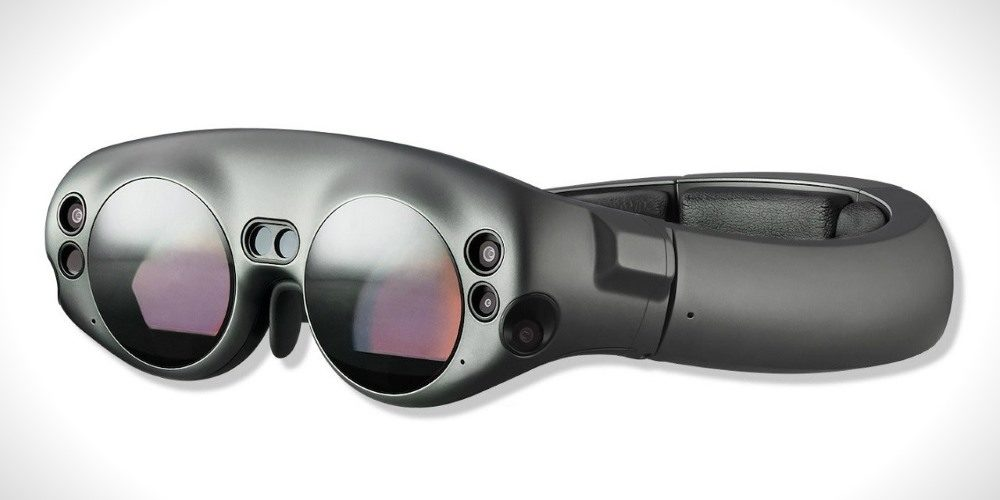
\includegraphics[scale=0.8]{Images/Estado del arte/magicleapone1.jpg}\\
        (a) Vista del casco completo
    \end{minipage}
    \begin{minipage}{0.5\textwidth}
        \centering
        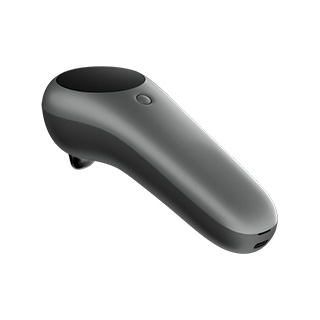
\includegraphics[scale=0.3]{Images/Estado del arte/magicleapone2.jpg}\\
       (b) Vista del mando
    \end{minipage}\\
    \caption{Dispositivo completo de las Magic Leap One\textsuperscript{\ref{magicLeaponeFotterImages}}.}
    \label{fig:vistasMagicLeapnOne}
\end{figure}

Por otro lado, utiliza una CPU (Unidad Central de Procesamiento) dos núcleos Denver 2.0 64-bit y cuatro núcleos ARM Cortex A57 64-bit, una Nvidia Pascal de 256 núcleos CUDA para la GPU (Unidad de Procesamiento Gráfico), tiene 128 Gigabytes como capacidad de almacenamiento y, por último, una batería de litio recargable que permite un uso continuado de 3 horas. 


%https://www.businessinsider.com/magic-leap-one-creator-edition-price-specifications-battery-life-release-date-2018-8?IR=T


\footnotetext[1]{
\label{magicLeaponeFotterSpecs}{Especificaciones obtenidas de \url{https://www.businessinsider.com/magic-leap-one-creator-edition-price-specifications-battery-life-release-date-2018-8?IR=T}.}}

\footnotetext[1]{
\label{magicLeaponeFotterImages}{Imágenes sacadas de \url{https://www.estiloextra.net/magic-leap-one-las-nuevas-y-prometedoras-gafas-de-realidad-aumentada/}.}}

\parindent=0em
\subsection{DAQRI Smart Helmet}
\label{subsec:DAQRISMART}
\noindent

%https://www.linkedin.com/pulse/daqri-smart-helmet-closer-look-nathan-gaydhani

El \textit{DAQRI Smart Helmet} (figura~\ref{fig:vistaDAQRIHelmet}) es un HMD enfocado al uso industrial, está formado por un dispositivo de realidad mixta sin cables integrado en un casco duro (cascos utilizados por ejemplo en la construcción). Ya que está pensado para un uso industrial está dotado de 4 cámaras para poder capturar todo el entorno, es decir, abarcar 360\degree .\\

\begin{figure}[H]
    \centering
    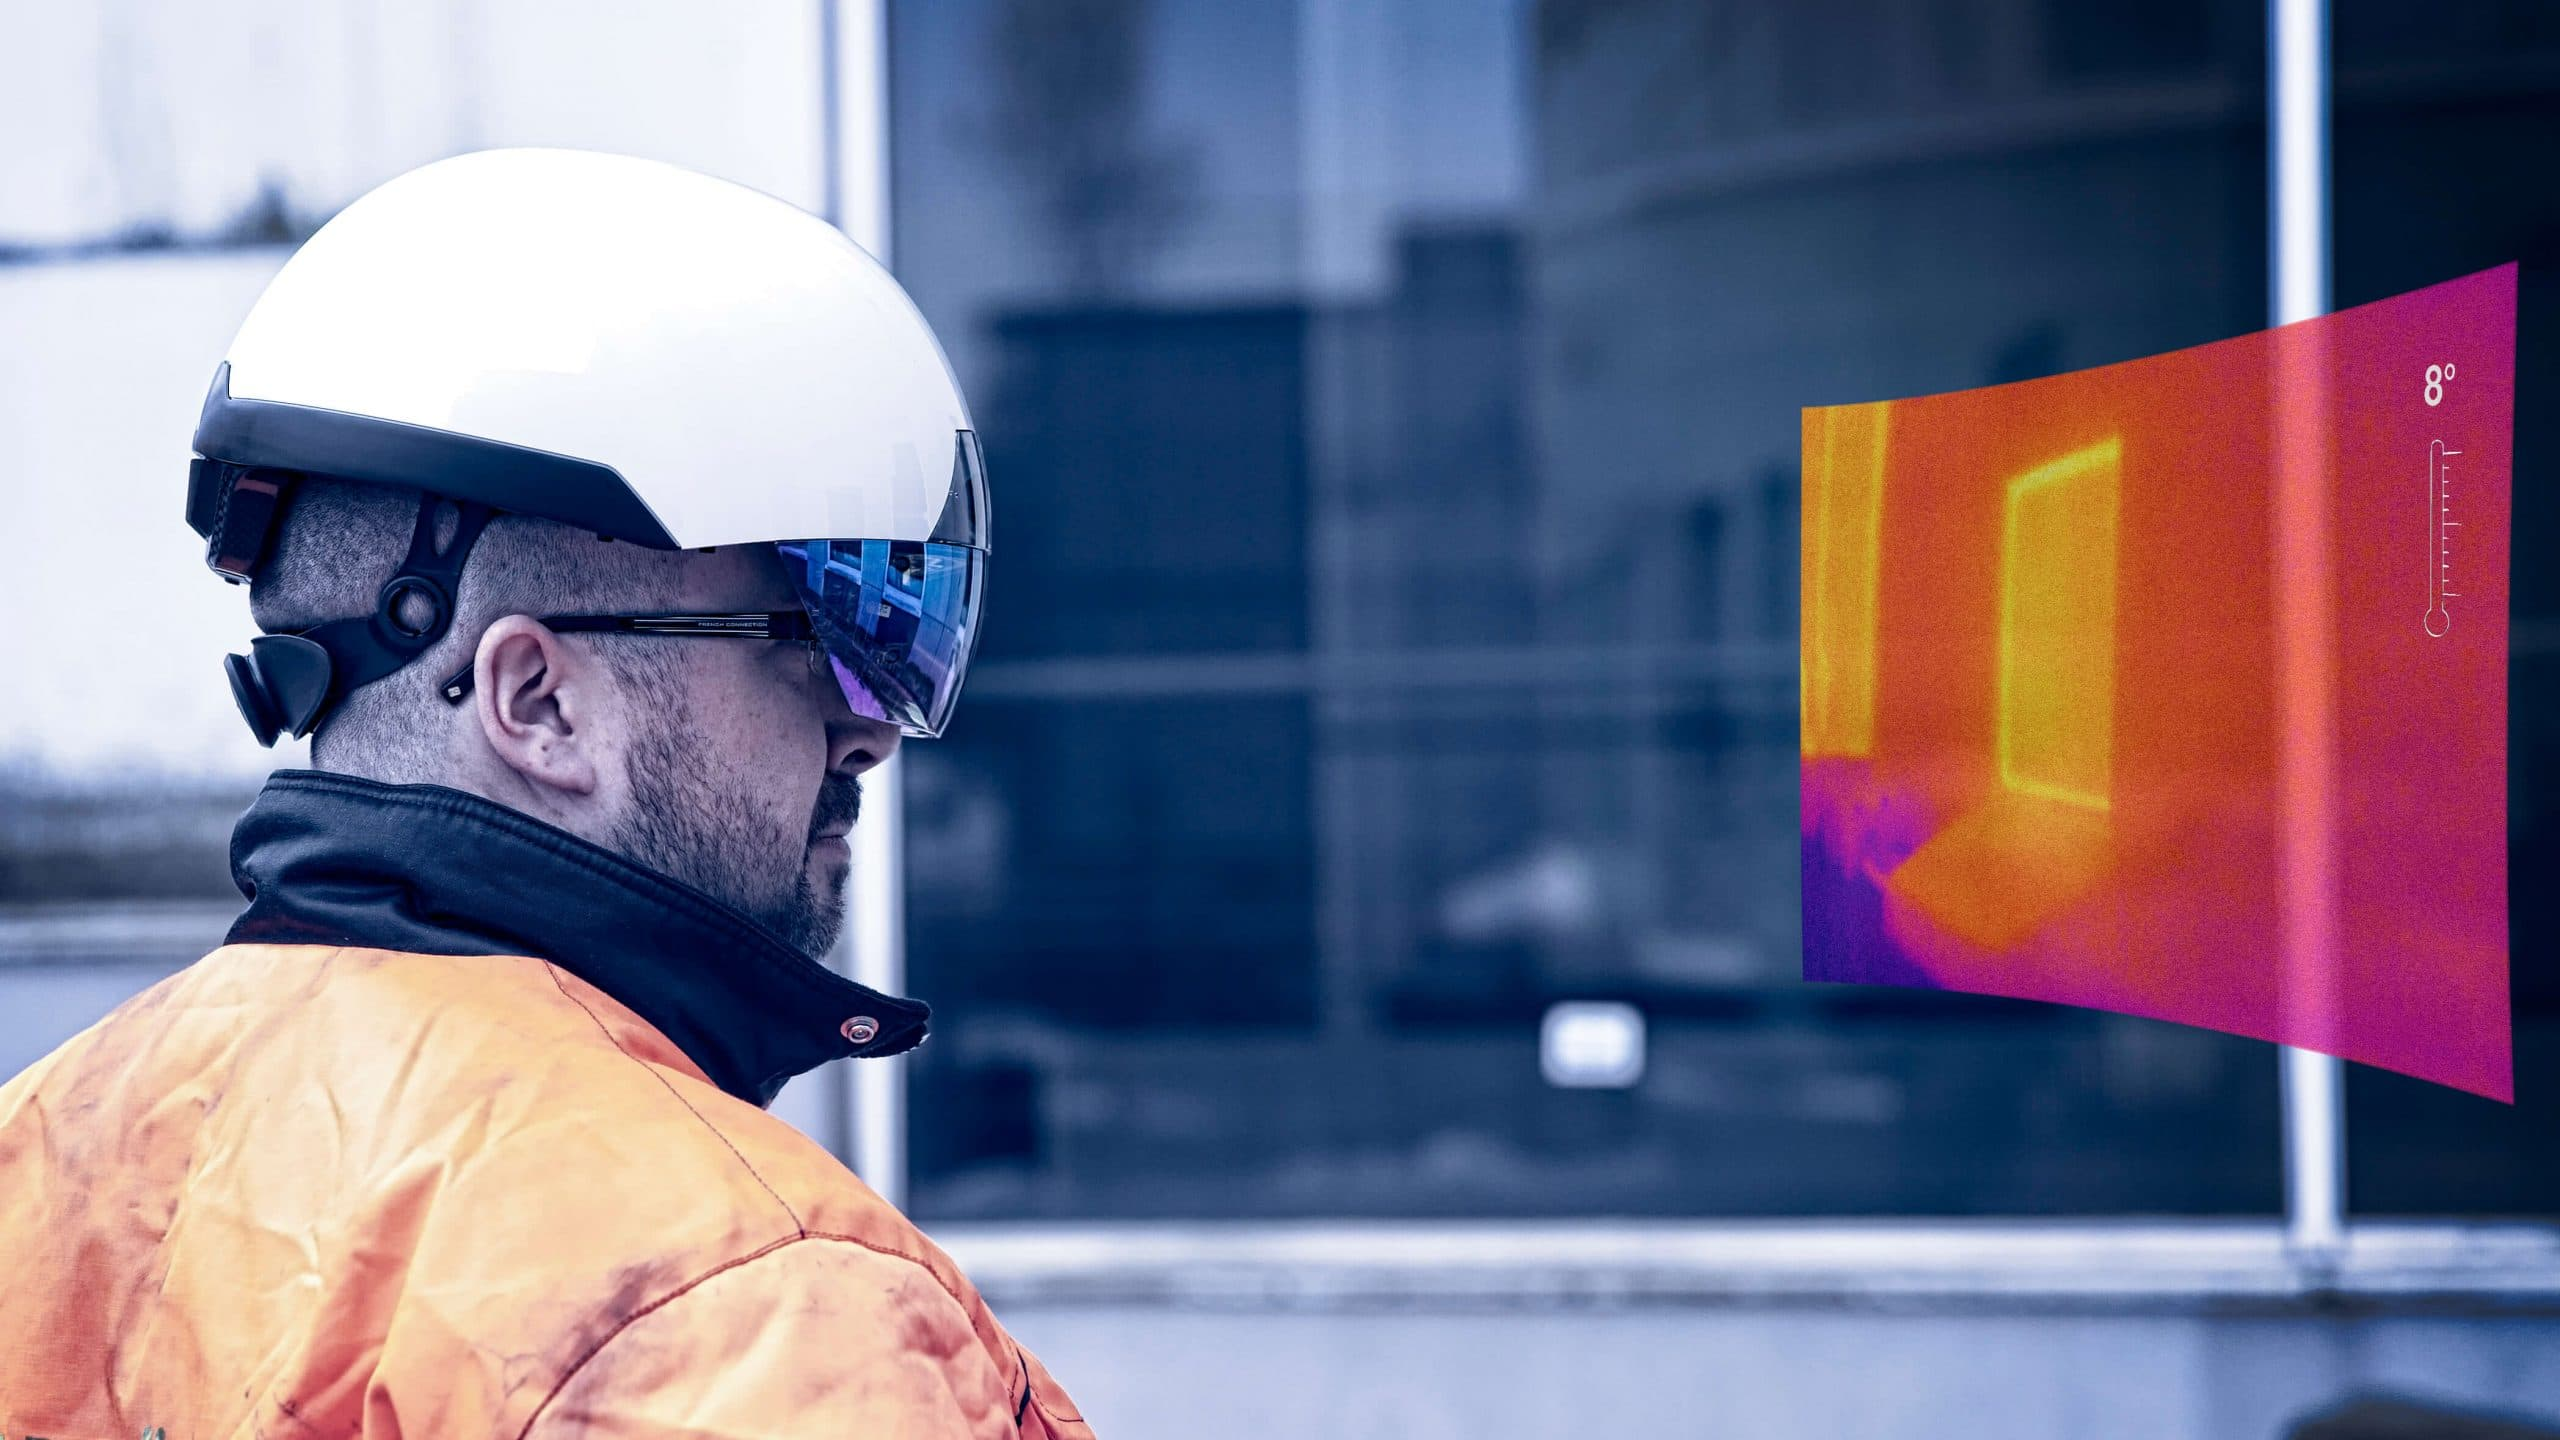
\includegraphics[scale=0.12]{Images/Estado del arte/daqrihelmet.jpg}
    \caption[Vista del \textit{DAQRI Smart Helmet}]{Vista del \textit{DAQRI Smart Helmet}\footnotemark.}
    \label{fig:vistaDAQRIHelmet}
\end{figure}

\footnotetext{Fuente: \href{https://www.stereoscape.com/blog/2017/04/25/daqri-smart-helmet-so-much-more-than-a-helmet/}{\nolinkurl{https://www.stereoscape.com/blog/2017/04/25/daqri-smart-helmet}}}


Con el objetivo de proteger al usuario en entornos industriales peligrosos, el dispositivo cuenta con una cámara termográfica (para poder controlar lugares potencialmente peligrosos debido a su temperatura) y barómetro para poder medir la presión del entorno.\\

Para el seguimiento, el \textit{DAQRI Smart Helmet} utiliza la tecnología SLAM y posee 6DoF para el movimiento y los giros del usuario. Del mismo modo, ya que el objetivo final es proteger al usuario, el dispositivo cuenta con reconocimiento de órdenes por voz y de control de movimientos de la cabeza para manejar el HMD, de esta forma se pueden tener las manos libres.\\


Finalmente, cabe recalcar que el casco goza de procesadores y un sistema operativo Android para ser totalmente independiente, también, utiliza unas baterías intercambiables de 5.700 miliamperios por hora y dispone de conectividad WiFi para poder comunicarse por vídeo en tiempo real remotamente con otros usuarios. El casco tiene un peso total de 1 kilo y~500 gramos y su precio actual es de~15.000 dólares.

%\footnotetext{\label{daqriImagefooter}{Imagenes obtenida de: %\url{https://www.stereoscape.com/blog/2017/04/25/daqri-smart-helmet-so-m%uch-more-than-a-helmet/}.}}




\parindent=0em
\subsection{HP VR1000-127il}
\noindent

Este \textit{HMD} de la empresa \textit{HP} salió al mercado en el año 2018, es un dispositivo dependiente de un ordenador compatible con la plataforma \textit{Windows Mixed Reality}. Este casco se conecta a dicho ordenador a través de una conexión 2 en 1 que combina un \textit{HDMI} 2.0 y \textit{USB} 3.0. \\

Las gafas \textit{HP VR1000-123il} (figura~\ref{fig:hpvr1000}) utilizan dos controladores inalámbricos (que se conectan mediante \textit{bluetooth}) para controlar el movimiento de las manos, estos controladores utilizan 2 pilas AA cada uno. El dispositivo tiene un campo de visión de 90º y una resolución de 1.440×1.440 píxeles por ojo (un total de 2.880x1.440 píxeles con ambos ojos), por otro lado, el casco cuenta con \textit{6DoF} y la \textit{IPD} no se puede regular. 

\begin{figure}[H]
    \centering
    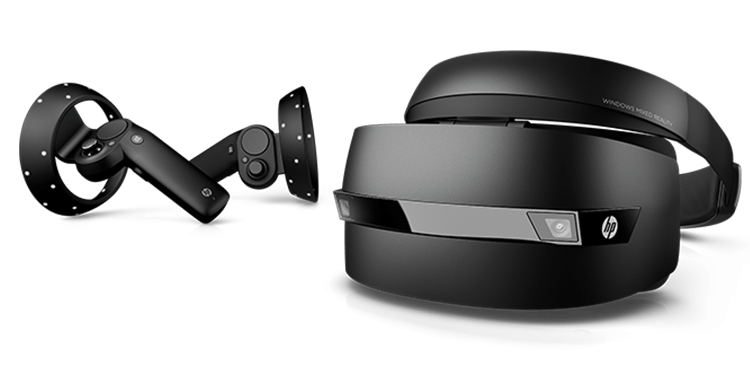
\includegraphics[scale=0.45]{Images/Estado del arte/HP VR1000.png}
    \caption{HP VR1000-123il y sus controladores.}
    \label{fig:hpvr1000}
\end{figure}

Finalmente, este \textit{HMD} no tiene un diseño centrado en su uso con gafas y tiene un peso de 834 gramos. 
\parindent=0em
\subsection{Asus HC102}
\noindent

Este dispositivo (figura~\ref{fig:asushc102}) apareció en el año 2018 de manos de la empresa Asus, al igual que las \textit{HMD Odyssey+} (punto~\ref{sec:odyssey}), es un dispositivo que requiere ser utilizado junto a un ordenador compatible con \textit{Windows Mixed Reality}, está dotado de sensores para calcular la orientación del usuario como giroscopio, acelerómetro, magnetómetro y sensor de proximidad.\\

\begin{figure}[H]
    \centering
    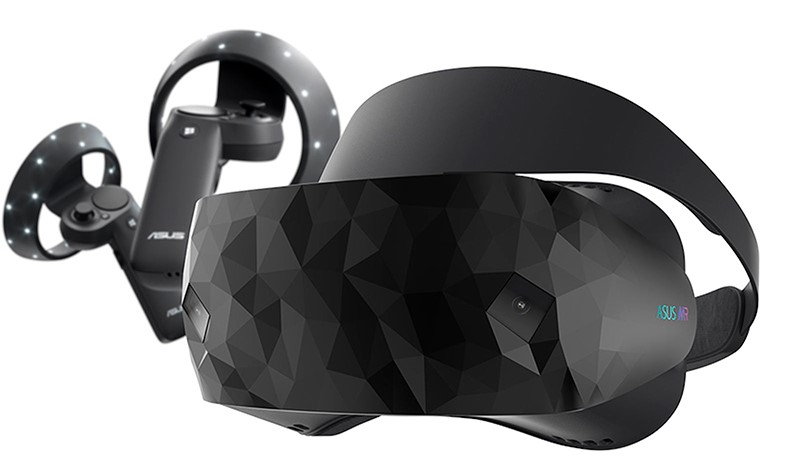
\includegraphics[scale=0.3]{Images/Estado del arte/AsusHC102.jpg}
    \caption[\textit{Asus HC102} al completo]{\textit{Asus HC102} al completo\footnotemark.}
    \label{fig:asushc102}
\end{figure}

\footnotetext{Fuente: \href{https://www.asus.com/Headset/ASUS-Windows-Mixed-Reality-Headset-HC102/specifications/}{\nolinkurl{https://www.asus.com/Headset/ASUSHC102/specifications/}}}

Este casco goza de un FOV de 105\degree , una resolución de 1.440x1.440 por ojo (2.880x1440 en total) y cuenta con dos mandos (cada uno de ellos con un sensor 6DoF) que funcionan con 2 pilas del tipo AA, es decir, 4 pilas AA en total.\\

Finalmente, este HMD permite regular la IPD entre 55mm y 71mm, tiene dos cámaras para hacer un \textit{tracking} de tipo \textit{inside-out} y un peso de 399 gramos.
\parindent=0em
\subsection{Acer AH101-D8EY}
\noindent

Este dispositivo de la marca \textit{Asus} fue lanzado al mercado en el 2017, para utilizarlo es necesario un ordenador compatible con \textit{Windows Mixed Reality}, en cambio, este \textit{HMD} se conecta al ordenador a través de conexión \textit{bluetooth} a diferencia de los otros cascos vistos que se conectan con un cable.\\

El campo de visión del casco es de 100º y respecto a la resolución, es capaz de mostrar 2.880x1.440 píxeles combinando los dos ojos (1.440x1.440 píxeles en cada ojo), además, la distancia interpupilar no es ajustable y viene configurada por defecto a 62mm.\\

Por otro lado, ya que se conecta mediante \textit{bluetooth} necesita una fuente de energía de 2 pilas tipo AA, del mismo modo, el dispositivo viene con dos controladores que igualmente funcionan con 2 pilas del tipo AA cada uno y tienen 6 grados de libertad. 
\parindent=0em
\subsection{Lenovo Explorer}
\noindent

La marca Lenovo puso a la venta el dispositivo \textit{Lenovo Explorer} (figura~\ref{fig:lenovoExplorer}) en el año 2017, es un casco de la realidad mixta que se utiliza a través de \textit{Windows Mixed Reality}, es decir, depende de un ordenador para ser utilizado. Este HMD se conecta a través de un cable en Y con conexión HDMI y USB~3.0 y goza de conexión \textit{bluetooth}.\\

Este dispositivo está dotado de sensor de proximidad, giroscopio, acelerómetro y magnetómetro, además, posee dos cámaras para realizar el \textit{tracking} \textit{inside-out}.\\

Por otra parte, tiene un FOV de 110\degree  y una resolución con ambos ojos de 2.880x1.440 píxeles (1.440x1.440 con cada ojo), tiene control de 6 grados de libertad  y su IPD no se puede ajustar viniendo fijo con un valor de 62mm. Este dispositivo no tiene tecnología \textit{hand tracking} ni \textit{eye tracking}, para sustituir el seguimiento de manos se utilizan dos controladores que funcionan con pilas del tipo AA. Su peso es de 380 gramos. 

%https://www.amazon.com/-/es/Lenovo-G0A20001WW-Explorer-Mixed-Reality-Auriculares/dp/B0764GKZ15


\begin{figure}[H]
    \centering
    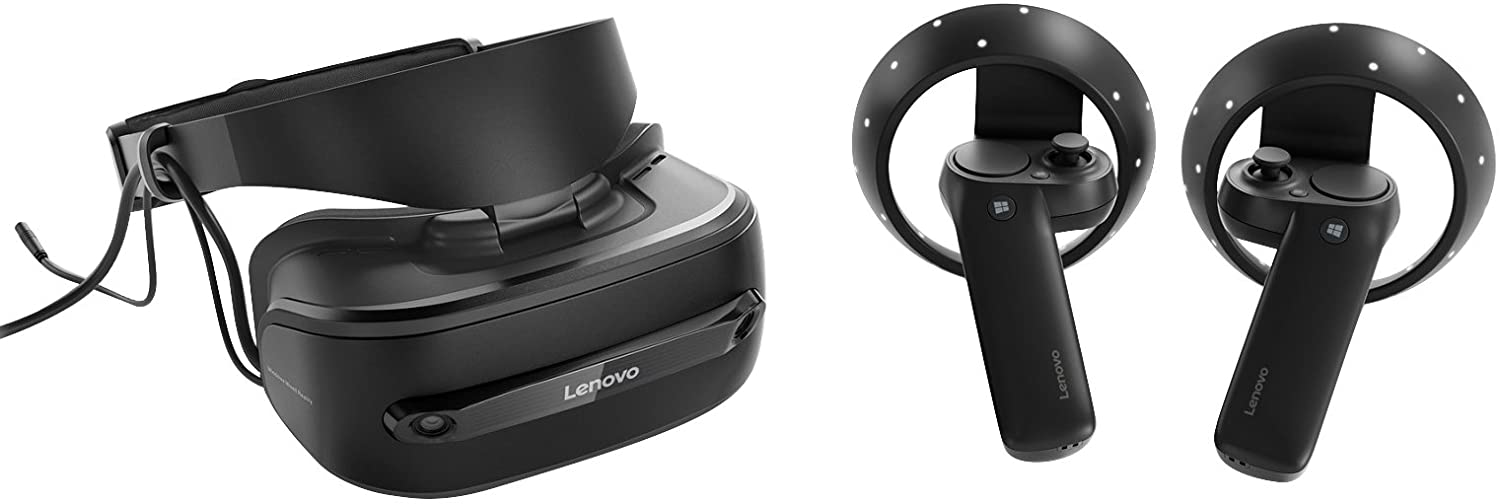
\includegraphics[scale=0.2]{Images/Estado del arte/lenovoexplorer.jpg}
    \caption[Lenovo Explore]{\textit{Lenovo Explore}r\footnotemark.}
    \label{fig:lenovoExplorer}
\end{figure}

\footnotetext{Fuente: \href{https://www.lenovo.com/es/es/smart-devices/virtual-reality/lenovo-explorer/Lenovo-Explorer/p/G10NREAG0A2}{\nolinkurl{https://www.lenovo.com/Lenovo-Explorer/p/G10NREAG0A2}}}

\parindent=0em
\subsection{Comparación de dispositivos}
\noindent

